\documentclass[11pt]{article}

\newcommand{\cnum}{CM146}
\newcommand{\ced}{Fall 2018}
\newcommand{\ctitle}[3]{\title{\vspace{-0.5in}\cnum, \ced\\Problem Set #1: #2}}
\usepackage{enumitem}
\newcommand{\solution}[1]{{{\color{black}{\bf Solution:} {#1}}}}
\usepackage[usenames,dvipsnames,svgnames,table,hyperref]{xcolor}
\usepackage{amsmath}
\usepackage{graphicx}
\usepackage[utf8x]{inputenc}
\usepackage{listings} %for listings of the source code


\renewcommand*{\theenumi}{\alph{enumi}}
\renewcommand*\labelenumi{(\theenumi)}
\renewcommand*{\theenumii}{\roman{enumii}}
\renewcommand*\labelenumii{\theenumii.}

\begin{document}
\ctitle{02}{Jonathan Chu}
\date{}
\maketitle
\vspace{-0.75in}

\section{(on CCLE)}
\section{(on CCLE)}

\section{Understanding Linear Separability}
\begin{enumerate}
\item %3a
\solution{
If $\delta$ = 0, we have:
$$y_i(\boldsymbol{w^Tx_i}+\theta) \geq 1$$
Trivially, this inequality holds when $sgn(y_i) = sgn(\boldsymbol{w^Tx_i}+\theta)$ and $|\boldsymbol{w^Tx_i}+\theta| \geq 1$.

The matching signs of $y_i$ and $\boldsymbol{w^Tx_i}$ indicate these values of $\boldsymbol{w}$ and $\theta$ satisfy equation (1). Therefore D is linearly separable.
}

\item %3b
\solution{
For $0 < \delta < 1$, it still holds that $sgn(y_i) = sgn(\boldsymbol{w^Tx_i}+\theta)$, meaning that D remains linearly separable, and $|\boldsymbol{w^Tx_i}+\theta| < 1$ for some i, which is not of any concern.

However, if the minimum $\delta \geq 1$, we have
$$y_i(\boldsymbol{w^Tx_i}+\theta) \geq c, \text{ } c \leq 0$$
and D is not linearly separable.
}

\item %3c
\solution{
The minimum value we can achieve for $\delta$ is 0. If this is the case, we seek $\boldsymbol{w}$ and $\boldsymbol{x}$ that satisfy the following:
$$y_i(\boldsymbol{w^Tx_i}+\theta) \geq 0$$
Trivially, $\boldsymbol{w} = \boldsymbol{0}$, $\theta = 0$ satisfy the above inequality yet clearly will not separate D.
}

\item %3d
\solution{
Trivially, we see that $\boldsymbol{w}=[1, 1, 1]$, $\theta=0$, $\delta=0$ is an optimal solution.

In fact, any solution with 
$$\delta = 0$$ 
$$|\boldsymbol{w^Tx_i}+\theta| = |w_1x_1 + w_2x_2 + w_3x_3 + \theta| \geq 1$$
$\implies |w_1 + w_2 + w_3 + \theta| \geq 1$ and $|-w_1 + -w_2 + -w_3 + \theta| \geq 1$

is optimal.
}
\end{enumerate}

\section{Implementation: Polynomial Regression}
\begin{enumerate}
\item %4a
By inspection, linear regression would not model the data very accurately. Although lines with negative slope on both the training and test data seem like they would perform moderately well, there would still be high training and test error, since the square distance from points to the line would be somewhat large for many of the data points. 


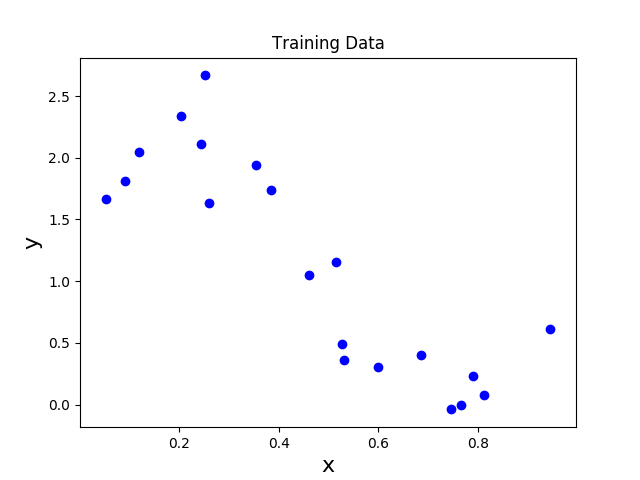
\includegraphics[width=\linewidth]{Training_Data.png}
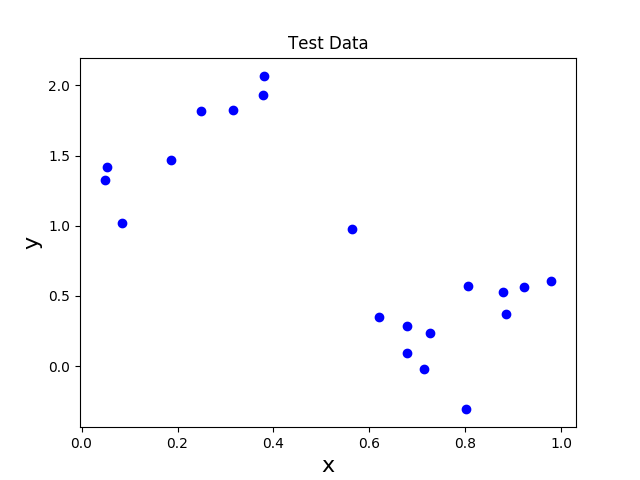
\includegraphics[width=\linewidth]{Test_Data.png}

\item %4b
\begin{lstlisting}
Phi = np.concatenate((np.ones(np.shape(X)), X), 1)
\end{lstlisting}

\item %4c
\begin{lstlisting}
y = np.dot(self.coef_, np.transpose(X))
\end{lstlisting}

\item %4d
Investigating linear regression...

	 --The model cost with zero weights is 40.233847


\begin{center}
\begin{tabular}{ |c|c|c|c|c| } 
 \hline
 $\eta$ & $\#$ Iter. & Final Coefficients & Final J($\theta$) & Time Taken (s)\\ 
 \hline
 0.00407 & 10000 & -9.4047e+18, -4.6523e+18 & 2.7109e+39 & 0.187604\\ 
 $10^{-4}$ & 764 & 2.4464, -2.8164 & 3.9126 & 0.0144\\ 
 $10^{-5}$ & 7020 & 2.4465, -2.8164 & 3.9126 & 0.1290\\ 
 $10^{-6}$ & 10000 & 2.2704, -2.4606 & 4.0864 & 0.1850\\
 \hline
\end{tabular}
\end{center}

For $\eta$ = 0.00407 and $10^{-6}$, the gradient descent algorithm stops when it reaches max iterations, meaning that it wasn't able to find a minimum. For 0.00407, the coefficients are very large, implying that the step size was too large, and the algorithm overstepped the minimum. 

For $10^{-4}$ and $10^{-5}$, the final coefficients match and the number of iterations is less than 10,000, meaning that in both cases, the algorithm found a minimum. However, we see that with $10^{-4}$, the algorithm converged after much fewer iterations, about a factor of ten less, so we know that the ideal step size is closer to $10^{-4}$. 

For $10^{-6}$, the final coefficients are close to the final coefficients for $10^{-4}$ and $10^{-5}$, but not quite there, implying that the step size was too small and the algorithm was taking too long to converge.

\item %4e 

Fitting with closed-form solution: \newline
	 --Final Coefficients: 2.446407, -2.816354 \newline
	 --Final value of objective function: 3.912576 \newline
	 --Time taken: 0.000306 \newline

The closed form solution method produces the same coefficients and final objective function value as gradient descent with a good step size. However, the time taken is much less than even the fastest gradient descent run, by a factor of about $10^2$.

\item %4f

Fitting with varied step size \newline
	 --number of iterations: 1779 \newline
	 --final coefficients: 2.446407, -2.816353 \newline
	 --final value of objective function: 3.912576 \newline
	 --time taken: 0.034152 \newline

The algorithm takes longer with varied step size than with a constant step size of $10^{-4}$, but takes less time than a constant step size of $10^{-5}$.

\item %4g

\item %4h
We prefer $E_{RMS}$ over $J(w)$ because it accounts for the number of training examples in addition to error. For less training examples and some given cost, $E_{RMS}$ will be higher, indicating more chance of overfitting. For the same cost but more training examples, $E_{RMS}$ will be lower, since the model is generalizing to more training data and thus has less chance of overfitting.

\item %4i
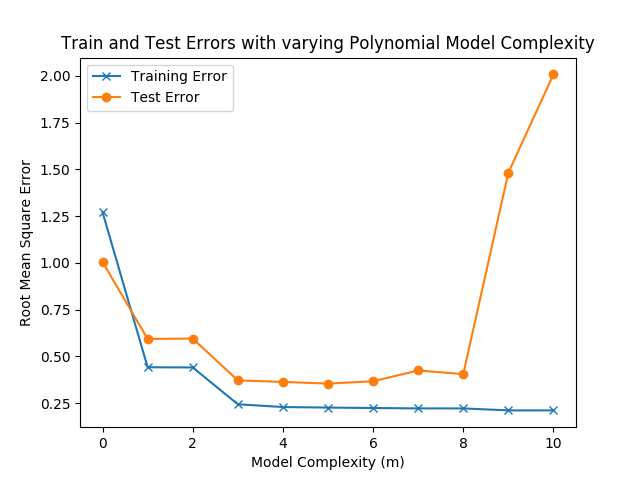
\includegraphics[width=\linewidth]{Errors.png}

The 10th degree polynomial clearly fits the \textbf{training} data best, with the lowest training error. However, the 9th and 10th degree polynomials overfit the data, as illustrated by the very high test errors and low train errors. 

As such, the best degree polynomial would be one with low training and test error, which appears to be somewhere in the range m=3 to m=6, which all seem to perform with similar error rates.

\end{enumerate}

\end{document}
